\section{Introduction}

Understanding and predicting the behavior of molecules and materials at the atomic level is fundamental to advancements across various scientific disciplines, including drug discovery, materials science, and catalysis \cite{wang2018silico, dominy2004native, cicaloni2019applications}. Accurate computational modeling allows researchers to explore chemical space, predict reaction outcomes, and design novel functional materials without the need for costly and time-consuming physical experiments.

At the heart of highly accurate computational methods lies quantum mechanics. Density Functional Theory (DFT) is a prominent approach that offers a favorable balance between accuracy and computational tractability for many systems \cite{engel2011density}. Instead of solving the complex many-body Schrödinger equation directly, DFT cleverly recasts the problem in terms of the electron density, $\rho(\mathbf{r})$. The core idea is that the ground state energy and all other ground state properties are unique functionals of the ground state electron density, $E_0 = E[\rho_0]$. In practice, DFT often relies on solving the Kohn-Sham equations, a set of single-particle equations that yield the electron density of the interacting system.

Despite the successes of DFT, a significant challenge remains in balancing computational accuracy with efficiency. The computational cost of DFT calculations scales cubically, limiting its application to relatively small systems or short simulation timescales \cite{engel2011density, cohen2012challenges}. Conversely, classical force fields, which use simplified, empirically parameterized functions to describe interatomic interactions, offer computational efficiency suitable for large-scale simulations (millions of atoms) and long timescales. However, these force fields often lack the necessary accuracy and transferability, especially for systems involving chemical reactions, complex electronic effects, or environments significantly different from those used in their parameterization \cite{herbers2013grand}.

To address the computational drawbacks of full DFT calculations, many machine-learning based approaches offer massive speedups. One landmark approach encodes molecules with an Atomic Environment Vector (AEV) representation, developed as part of the ANI framework, specifically the ANI-1 potential described by Smith et al.. \cite{smith2017ani} The ANI-1 potential and its associated AEVs demonstrated the ability to achieve near-DFT accuracy for predicting molecular energies and forces but at a significantly reduced computational expense, comparable to traditional force fields. The AEVs provide a fixed-size, symmetry and permutation-invariant descriptor of an atom's local chemical environment, making them suitable inputs for simpler neural network models by essentially enforcing a hard prior that the local environment contains all relevant energy information. The approach has been shown to be effective and easily extensible for a wide range of molecular systems, including organic molecules and biomolecules, and has been eimproved for larger systems and applications. \cite{devereux2020extending}

Here, I try to refine the existing ANI-1 potential to improve its performance on a specific class of molecules, namely, small organic molecules. I use the ANI potential as inspiration to adapt different model architectures to a subset of the GDB dataset \cite{ruddigkeit2012enumeration} comprised only of small molecules with the atoms Hydrogens, Oxygens, Carbons, and Nitrogens. The goal is to achieve a more accurate and efficient model for predicting molecular properties, particularly for small organic molecules.

\section{Methods}

I explored several neural network architectures and training strategies to refine the ANI potential for small organic molecules. The primary goal was to enhance the model's ability to predict molecular properties with higher accuracy while maintaining computational efficiency. To achieve this, I experimented with a variety of architectural modifications and training methodologies. All models were trained using the exact same atomic environment vector (AEV) representation implemented with the torchani package. \cite{gao2020torchani} The output of the model was a single scalar value representing the predicted molecular energy.

All architectures were built to be duplicated for use on each atom. The main ones tested included the incorporation of multi-head self-attention layers \cite{vaswani2017attention} before feedforward layers to capture complex and long-range interactions in the atomic environment. Residual connections were also evaluated to facilitate gradient flow and mitigate the vanishing gradient problem, which is particularly important for deeper networks. Various activation functions were also evaluated, including ReLU, GELU \cite{hendrycks2016gaussian}, and CELU, to determine their impact on model performance and convergence speed.

The dataset used for training and evaluation was split into 80\% training, 10\% validation, and 10\% testing to ensure a fair evaluation of the model's performance. To further enhance the robustness of the evaluation process and mitigate overfitting, I employed K-Fold cross-validation with $k=3$. This approach allowed the model to be trained and validated on multiple subsets of the data, providing a more comprehensive assessment of its generalization capabilities.

 The primary evaluation metric for the models was the Mean Absolute Error (MAE) in kcal/mol, which directly reflects the accuracy of the predicted molecular energies. This metric was chosen because it provides an intuitive measure of the average deviation between predicted and true values, making it suitable for assessing the performance of regression models in this domain.

All training was conducted using the Adam optimizer, which is well-suited for handling sparse gradients and adaptive learning rates. Hyperparameters, including batch size, learning rate, number of epochs, and L2 regularization strength, were manually tuned through an iterative process to optimize the model's performance. Early stopping was employed based on the validation loss to prevent overfitting and ensure that the model did not continue training once its performance on unseen data began to degrade.

To accelerate computation and enable the training of more complex models, all computations were conducted on an NVIDIA RTX3050 laptop GPU through a windows subsystem for linux on the x86-64 architecture with 32GB of RAM. This setup provided sufficient computational power to handle the dataset and the computational demands of training neural networks of this. The final model was selected based on the lowest validation MAE observed during training. Once selected, the model was evaluated on the held-out test set to report its performance, ensuring that the reported results reflect its ability to generalize to unseen data.

\section{Results}

The best model architecture was a set of four simple Feedforward networks with a single hidden layer of 128 weights that used a ReLU activation function, making up 197636 learnable parameters in total.

\begin{figure}[h]
    \centering
    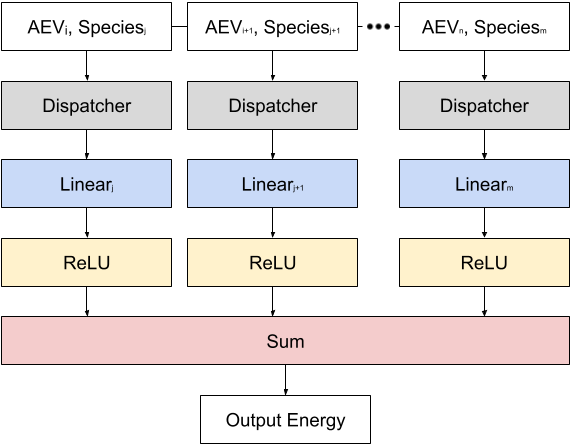
\includegraphics{figures/bioe142.png}
    \caption{Performance comparison of the best model architecture on the test set.}
    \label{fig:performance_comparison}
\end{figure}

\section{Discussion}
\lipsum[5]

potential limitations and improvements: not investigated for label imbalance, not investigated for almost-leakage like dataset behaviour, many training adjustments could be made, could use different networks for each atom like they did in the schrod. paper that improved on ani.

\section{Code Availability}

All code, data, and pytorch models used in this project are publicly available on GitHub under the MIT license at \url{https://github.com/Qile0317/bioe142-final-project}.

\printbibliography[heading=bibnumbered]
